
\section{Unanswered questions and new physics quests}\label{sec:THquest}

In the case the new boson discovered in July 2012 
really is a Standard Model Higgs boson, there would
be no more arguments to contradict the 
validity of the Standard Model, at least 
as an {\it effective theory} at low energies. Indeed many facts, both 
in theory and experiments, hints that the Standard Model,
despite is great success in describing the interaction
of fundamental particles, might be just an approximation
at low energy regimes of a more complete theory.

One of the principal objections to the Standard Model as 
``the final theory'' is the high number of arbitrary parameters 
of the theory. In fact, 19 parameters are needed to fit 
data from experimental observations. 
Three of them  are the couplings of the gauge groups 
$g, g', g_s$ for the electroweak and strong
interactions respectively, also written as: 
\begin{equation}\label{eq:couplings}
\alpha_{EM} = \dfrac{e^{2}}{4\pi} =  \dfrac{g^{2}\sin^{2}\theta_{W}}{4\pi}, 
\quad \sin^{2}\theta_{W} = \dfrac{(g')^{2}}{g^{2}+(g')^{2}}  ,\quad 
\alpha_{s}=\dfrac{g_{s}^{2}}{4\pi}.
\end{equation}
Then, 13 parameters are associated with the nine charged 
fermion masses and the four parameters of the CKM matrix 
(three quark-mixing angles and one phase), 
two are needed to describe the Spontaneous Symmetry Breaking mechanism, 
i.e. the Higgs vacuum expectation value $v$ and 
the quartic coupling constant $\lambda$, and the last one is the 
QCD $\theta$ parameter, introduced in the lagrangian to account
for CP violation. Additionally, if neutrinos are massive 
(as it is almost certain from neutrino oscillation observations, 
see e.g. \cite{Langacker:817840}) there will be even more arbitrary 
parameters describing their masses and their mixing. 
Furthermore, massive neutrinos cannot exist in the Standard
Model, where only left-handed neutrinos are predicted and thus
no Dirac mass term can appear\footnote{A way out of this
problem postulates a new type of neutrinos, namely 
{\it Majorana neutrinos}, in contrast to {\it Dirac neutrinos}.}.


%If, based on these considerations,  one assumes that 
The arbitrariety of parameters, and in particular of the
fermion masses, introduces what goes under the name of
{\it naturalness problem}. A ``natural'' theory is
characterized by free parameters with values of, more or
less, the same order of magnitude. This does not happen in
the Standard Model, where the top quark, as an example,
has a mass $\sim 10^5$ larger than the up quark.
This issue further develops as follows. If the 
Standard Model is valid only up to  an energy scale 
$\Lambda$ (which, if it's the Planck scale
at the far right of Figure~\ref{fig:scales}, differs
from the electroweak scale by $\sim 10^{17}$!), 
then the scalar Higgs boson mass 
should encounter radiative corrections from 
vacuum polarization diagrams (like the one in Figure~\ref{topLoop}) 
of the order of $\Lambda$ giving to the mass the 
value: %~\cite{dawson-1997}:
\begin{equation}\label{eq:higgsMass}
M_{H}^{2} \sim M_{H_{0}}^{2} 
+ \dfrac{\lambda}{4\pi^{2}} \Lambda^{2} 
+ \delta M_{H}^{2}. \end{equation}
If the mass counterterm $\delta M_{H}^{2}$ does not 
cancel the quadratically divergent contribution and 
if the cutoff scale is chosen as the Planck scale, then
\begin{equation}
M_{H}^{2} \sim 10^{32},\end{equation} 
i.e. many orders of magnitude bigger than the experimentally 
measured value coherent with the Standard Model 
and with the unitarity constraint. This  
is the \textit{hierarchy problem}, and 
could be fixed within the Standard Model by 
choosing a fine-tuned mass counterterm, a 
solution considered not really elegant also 
because fine tuning will be required for every 
order in the perturbative expansion\footnote{This 
problem does not arise with loop corrections to 
fermion masses, which are protected by the chiral 
symmetry, nor with gauge boson masses,
which are protected by gauge invariance. It
is, actually, a general issue for elementary scalar particles
like the Higgs boson.}. %and that's the reason why fermion masses are said to be ``natural''.} 


\begin{figure}[htb]\begin{center}
%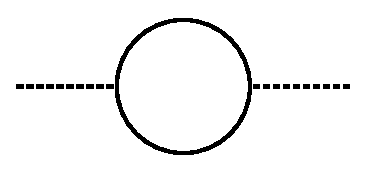
\includegraphics[width=.2\textwidth]{theory/figures/loop1}
\subfigure{ \def\svgwidth{0.25\textwidth}
\input{theory/figures/mod_loop1.eps_tex}}
\caption{Example of vacuum polarization diagram 
  for the Higgs boson involving the top quark loop.}
\label{topLoop}\end{center}\end{figure}
%This argument looks the same of what made physicists pass from Fermi theory to Standard Model. In fact at that time the Fermi point like interactions were a good description of weak scattering processes of fermions $f+f\rightarrow f+f$, but the unitarity  predicted that at an energy $E_{crit} \sim 600$ GeV the theory would become inconsistent. Then it was found that new physics (the vector bosons of the Standard Model) was needed already from an energy scale about 100 GeV, maybe due to the small coupling constant of weak interaction. Now, the scattering process $W+W\rightarrow W+W$ has a scattering amplitude growing linearly to the self-coupling constant of the Higgs field $\lambda$. The formula for the critical energy is now related to the Higgs mass as \cite{Ho-Kim} $$\dfrac{E_{crit}}{v} = \exp\bigg(\dfrac{4\pi^{2}v^{2}}{3M_{H}^{2}}\bigg),$$ which for an higgs Higgs mass less than 150 GeV gives $E_{crit} \sim 10^{18}$, thus making the Higgs model valid up to that scale. However for an heavier Higgs with a mass about 700 GeV, such critical energy goes down to $10^{3}$ GeV.  It is to remark that in the electroweak interactions the Higgs contribution to radiative corrections is very low since is denoted by a logarithm function, thus giving low variations and not affecting the precision electroweak data. The meaning of this is, whatever the critical energy value will be, the Standard Model is an effective theory embedded in a more fundamental theory with $E_{crit}$ acting as a cutoff.

\begin{figure}[h!tb]\begin{center}
        \subfigure{ %\def\svgwidth{0.9\textwidth}
\input{theory/figures/mod_scales.eps_tex}}
	\caption{Typical length and energy scales
          of some of the fundamental parameters
          of the Universe.\label{fig:scales}}
\end{center}\end{figure}

Another disturbing feature of the Standard Model as it is 
is the lack of theoretical explanation for the generations 
of quarks and leptons to be exactly three, as suggested
(under certain assumptions) by precision measurements 
performed at LEP at the $Z$-pole ($\rts\sim 91$~\gev). 
From QCD comes the only constraint for quark generation
to be less that nine.

Cosmology and cosmological observations also challenge 
the Standard Model. The reason for the baryon-antibaryon 
asymmetry is still not understood although we know 
that it is connected to  CP violation\footnote{The CP violating 
phase introduced in the CKM mechanism cannot, however, 
account for the total baryon-antibaryon asymmetry measured.}. 
Besides, astronomical observations~\cite{Ade:2013zuv} 
tell us that the energy density of the 
Universe is made only for a 4-5\% of ordinary baryonic 
matter, the other components being dark matter (20-25\%) 
and dark energy (70-76\%). Dark matter is non-baryonic 
matter that interacts only weakly and gravitationally and,
therefore, cannot be observed with telescopes but it
is revealed by its gravitational interaction with ordinary 
matter in space. 
It is now believed that Dark Matter is composed  of 
Weakly Interacting Massive Particles (WIMPs) whose 
masses range from a few GeV to a few TeV and  are 
not predicted by the Standard Model. Dark energy instead is 
even more mysterious and maybe new physics discovery will 
give some hints for its interpretation.

Another topic making the Standard Model likely to 
need improvements is the desire to go further in 
the unification of theories. Gravity is not 
implemented in the Standard Model, nor is available
a widely accepted quantum theory of gravity.
This is acceptable at the electroweak scale of 
few hundreds of GeV where the strength of gravity
is negligible, but its effect should become relevant 
going up to the Planck scale $\Lambda \sim 10^{19}$ GeV. 
Also, electroweak and strong forces forming the Standard 
Model gauge group $SU(2)_{L}\otimes U(1)_{Y}\otimes SU(3)_{C}$ 
are expected to unify at high energy since their coupling 
constants are running constants dependent on the energy 
scale (Figure~\ref{running}).
\begin{figure}[htb]\begin{center}
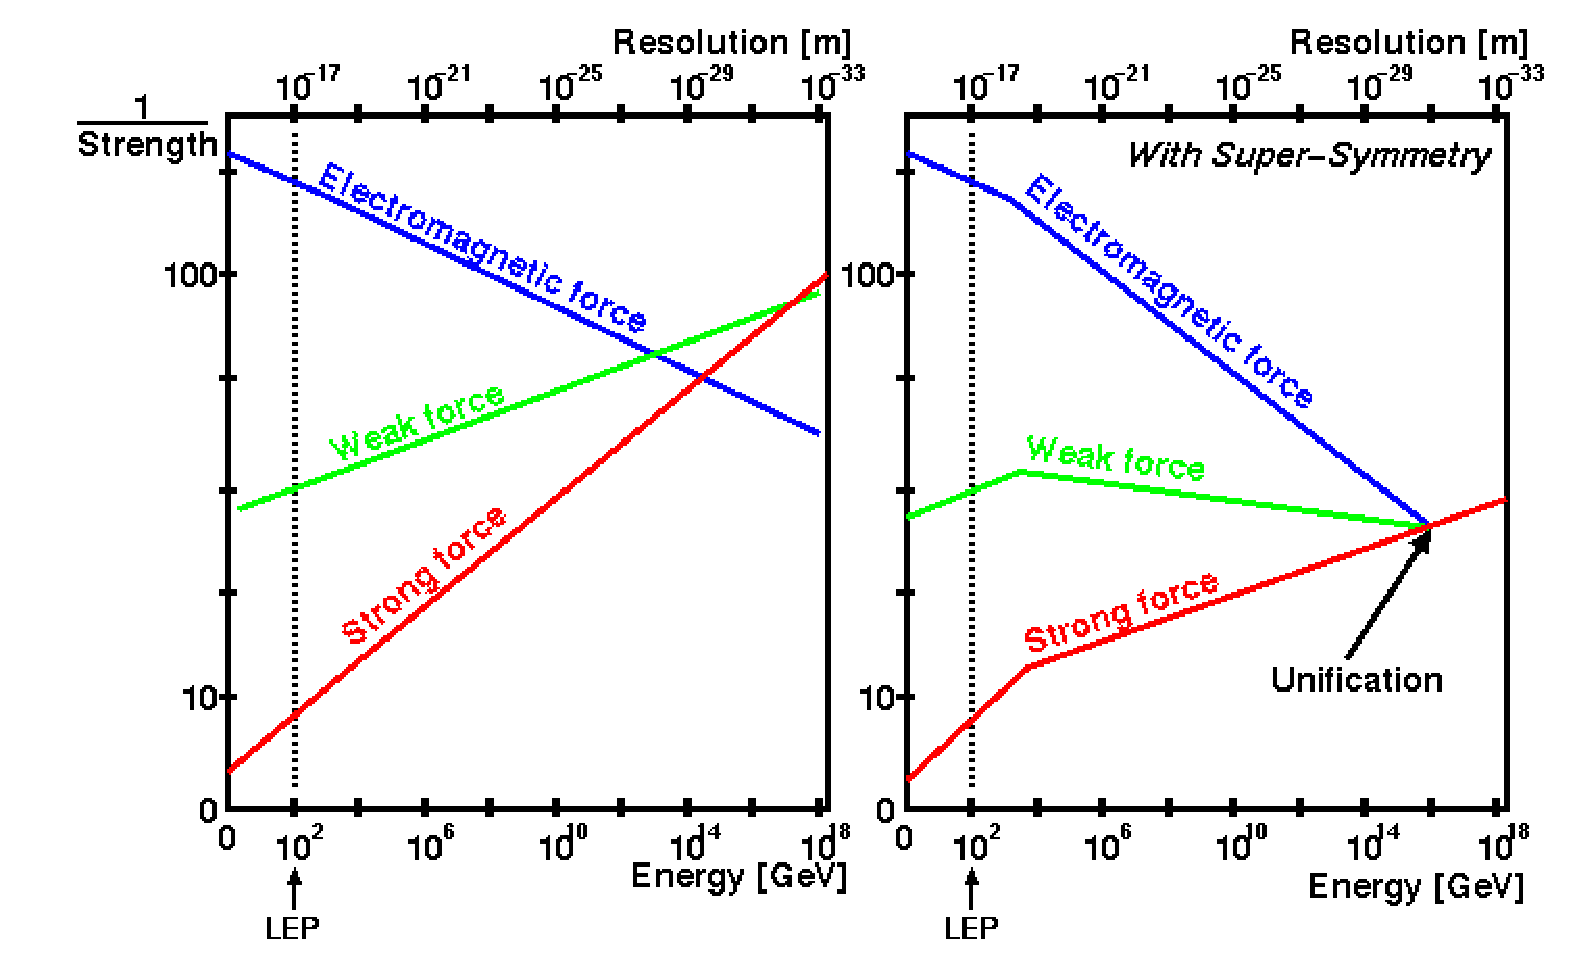
\includegraphics[width=.8\textwidth]{theory/figures/running_coupling}
\caption{Running coupling constants $\alpha^{-1}_{i} = g^{2}_{i}/(4\pi)$ in the Standard Model (left) and 
in a hypothetical Supersymmetric Model (right, see Section~\ref{sec:susy}) 
as functions of the renormalization scale (picture from \url{http://scienceblogs.com},
original credits unknown). The energy scale explored at LEP is marked
on the two figures and corresponds to $10^2$~\gev. The LHC is able to
go just one order of magnitude further.}
\label{running}\end{center}\end{figure}

In the following some ``beyond-Standard Model'' (BSM) theories
proposed to solve some of the shortcomings of the SM
are briefly discussed.



\subsection{Fourth generation SM4}\label{sec:sm4}

One of the simplest modifications to the Standard Model
is the addition of a fourth generation of fermions, a
scenario referred to as SM4~\cite{Holdom:2009rf}. 
This does not contradict the precision measurements of the $Z$
boson decay width performed at LEP since the fourth neutrino
might have a mass $m_{\nu_4}>m_{Z}/2$.

The new fermions are sometimes called $f_4$ ($f=u,d,l^{-},\nu$)
or, more frequently, $t', b', \tau', \nu_{\tau}'$. In the
Standard Model lagrangian additional Yukawa couplings appear
and the CKM matrix is extended to a $4\times 4$ matrix that
transforms the weak eigenstates into the mass eigenstates.
This introduces three complex phases allowing for more
sources of CP violation\footnote{The $3\times 3$ CKM
matrix has only one complex phase.}. Combining experimental
measurements and unitarity constraints, the elements of
the SM4 CKM matrix can be evaluated~\cite{Lacker}. It
can be intuitively expected that the fourth generation mixes
primarily with the third generation, but this is not always 
the case. If it is further
assumed that the mass splitting between the two new quarks
$t'$ and $b'$ is lower than the value of the $W$ boson mass,
the decay $t'\to Wb'$ is not allowed and the fourth generation
quarks will decay into a $W$ boson and a standard model quark,
according to the matrix elements $|V_{qt'}|$ ($q=u,c,t$) 
and $|V_{qb'}|$ ($q=d,s,b$).

After the discovery of a Standard Model-like Higgs boson,
the measurements performed of its cross section and decay 
branching ratio apparently rule out the possibility
of extra quarks that receive mass through the Yukawa couplings
with the Higgs doublet~\cite{Djouadi:2012ae}.
Indeed the Higgs production through gluon-gluon fusion
in the Standard Model would be 9 times larger than
the measured value due to the additional contributions,
but there are still some models that allow 
for a chiral fourth generation~\cite{Cetin:2011aa}.



\subsection{Supersymmetry}\label{sec:susy}

Since Supersymmetry~\cite{Wess:320631} is one of the most popular
BSM scenarios, having many trustful supporters even
now that after the first LHC run no trace of it
has been found, a brief explanation of its concepts
is included in this dissertation.

The basic idea is to postulate the invariance 
of the theory under a symmetry operation which 
trasforms fermionic fields into bosonic fields 
(and viceversa), called \textit{supersymmetry} (SUSY). 
In this theory to each fermionic or bosonic 
degree of freedom of the Standard Model is associated a 
``superpartner''. These superpartners have all 
of the quantum numbers identical to the corresponding 
Standard Model particles, except for the spin quantum number 
transformed as $s' = |s - 1/2|$. Thanks to the 
presence of superpartners, the Fermi statistics 
allows to write the new version of Equation~\ref{eq:higgsMass} as:
\begin{equation}
\label{eq:higgsMassSUSY}
M_{H}^{2} \sim M_{H_{0}}^{2} + \dfrac{g_{F}^{2}}{4\pi^{2}} (\Lambda^{2} + m_{F}^{2} ) - \dfrac{g_{S}^{2}}{4\pi^{2}} (\Lambda^{2} + m_{S}^{2} ),
\end{equation} 
where the subscripts $F$ and $S$ indicate respectively 
fermionic and scalar degrees of freedom. If $g_{F} = g_{S}$ 
and masses are equal as in an unbroken supersymmetry scenario, 
the $\Lambda^2$ terms cancel and the hierarchy problem is solved. 
However, since no superpartners of known particles 
have been observed,  supersymmetry must be a broken 
symmetry and sparticles masses have to lie in an 
energy range not yet accessed by experiments.

%The simplest and most popular supersymmetric model is called the Minimal Supersymmetric extention of the Standard Model (MSSM). In the MSSM, $SU(2)_{L}\otimes U(1)_{Y}\otimes SU(3)_{C}$ gauge symmetries are still valid, but particles are now organized in \textit{Chiral Superfields} (formed by a complex scalar field and a fermion field with two components) and \textit{Vector Superfields} (made of a massless gauge field and two-component fermion field named \textit{gaugino}). Even if the scalar superpartners of fermions do not feature handedness, the chirality is formally assigned as the one of the standard particles in the supermultiplet. Then, for every family of quarks and leptons of the SM, a superfield made of an $SU(2)_{L}$ doublet of fermions and an $SU(2)_{L}$ doublet of scalars is defined ($\hat Q_{1,2,3}$ for quarks, $\hat L_{1,2,3}$ for leptons), as well as one superfield of right-handed anti-leptons and anti-sleptons ($\hat E_{1,2,3}$) and two superfields of right-handed anti-quarks and anti-squarks ($\hat U_{1,2,3}$ and $\hat D_{1,2,3}$). There are then two other Chiral Superfields in the Higgs sector ($\hat H_{u,d}$) and three Vector Superfields made of the gauge bosons and their relative superpartners ($\hat{G}^{a},\ \hat{W}^{i},\ \hat{B}$). 
%As can be seen in the summary of the MSSM supermultiplets in Table \ref{tab:supermultiplet}, an additional Higgs doublet needs to be postulated. The reason is that while in Equation \ref{eq:higgsMassSUSY} the term from scalar squarks cancels, in the similar equations for the fermions masses, where anomalies are automatically  cancelled within the SM, the newly introduced term from the Higgsino fermionic field remains. Thus another Higgs doublet with opposite $U(1)$ quantum number is defined. Furthermore, having two Higgs doublets is in general also required in order to give masses to both up and down type quarks in Supersymmetric theories. The two Higgs doublets with their eight components yield four extra bosons with respect to the SM, i.e. we get five physical Higgs bosons ($h^{0}, H^{0}, A^{0}, H^{\pm}$) and the relative superpartners, the fermionic Higgsinos. Gauginos mix  with Higgsinos resulting in the eight mass eigenstates: $\tilde{\chi}^{\pm}_{1,2}$ (the \textit{Charginos}) and $\tilde{\chi}^{0}_{1,2,3,4}$ (the \textit{Neutralinos}). After defining the superfields it is possible to construct the Lagrangian of the MSSM; a very clear step-by-step  pedagogical description for this task is given in Ref.~\cite{Martin}.

Supersymmetry also provides a natural candidate
for Dark Matter, the Lightest SUSY Particle (LSP), 
which, in a {\it R-parity}\footnote{The quantum number 
\textit{R-Parity} is defined as $R \equiv (-1)^{3(B-L) + 2s}$
to prevent lepton and baryon numbers from being violated.
It has value $+1$ for all Standard Model particles 
and $-1$ for their superpartners.} 
conserving scenario~\cite{Martin:1997ns},
would be stable, weakly interacting and neutral.



\subsection{Composite and Little Higgs}\label{sec:littlehiggs}

The SSB mechanism, described previously in Section~\ref{sec:THlagr},
does not apply only to the Standard Model. It is, indeed,
a feature of many models. In general, when a symmetry is
spontaneously broken, {\it Goldstone bosons} (scalar, massless particles)
arise~\cite{PhysRev.127.965}, like excitations of the field.
The Goldstone boson can aquire mass if the symmetry is not exact
and is both spontaneously and explicitly broken. In this case
the boson is called {\it pseudo-Goldstone bosons} (PGB).
To each generator of the broken symmetry corresponds a
(pseudo-)Goldstone boson. In the Higgs mechanism, where the
$SU(2)_L\otimes U(1)_Y$ symmetry is gauged, three out of four
Goldstone bosons are ``eaten'' by the $Z$ and $W^{\pm}$
bosons, while the fourth is what then becomes the Higgs boson.

A nice example of a pseudo-Goldstone boson is the pion,
which was considered the responsible for quark masses. 
%when only two generations were known.
In QCD the flavor chiral symmetry of the Lagrangian is 
%decomposed in the groups:
%\begin{equation}\label{eq:qcdchiral}
%SU(N)_L \otimes SU(N)_R  \otimes U(1)_V \otimes U(1)_A,
%\end{equation}
%where besides the doublet left- and right-handed 
broken spontaneously, generating three
massless scalar bosons. The further explicit symmetry breaking
operated by the quark masses gives mass also to the 
pseudo-Goldstone bosons which is, however, much smaller than
the other mesons' masses. The three pseudo-Goldstone bosons 
are the $\pi^{\pm}$ and $\pi^0$ particles. %, but the argument can be extended to the complete model with three generation where 
However, the pion is not a fundamental particle as
it was believed before the idea of quarks was first
proposed but is, indeed, composed by quarks. 


% The chiral symmetry transformation can be divided into a component that treats the left-handed and the right-handed parts equally, known as vector symmetry, and a component that actually treats them differently, known as axial symmetry

In a similar way one can construct 
a class of BSM theories that go under the name
of {\it strong EWBS} (from ElectroWeak Symmetry Breaking).
These scenarios predict either no Higgs boson at all 
(as in {\it technicolor})
or a light pseudo-Goldstone Higgs bosons. The latter
is the case for {\it composite Higgs} models~\cite{Vecchi:2013bja,delAguila:2010vg}, 
where the mass of the Higgs boson is now naturally low and
hence there is no hierarchy problem to worry about.
What happens here is that up to a certain energy scale
(imposed to be ``far'' from the electroweak scale), the
Higgs does not show its composite nature (these new strong
constituents being, for now, undefined). There are then
in the theory two sectors: one well described by 
the Standard Model gauge and particle fields (the 
{\it elementary} sector), and another ``strongly'' coupled
containing the Higgs field and new heavy resonances 
({\it composite} sector).
In the composite sector a global symmetry is spontaneously 
broken and then, thanks to small mixing with the
elementary sector, it is also explicitly broken, giving
a pseudo-Goldstone bosons. 

%AAAAAAAAAAAAAAAAAAAAAAAAAAAAAAAAAAAAAA
Many models developed from the composite Higgs scenario,
such as Little Higgs models. predict
exotic heavy quarks~\cite{Contino:2008hi,Mrazek:2009yu}.


\subsection{Extra-dimensions}\label{sec:extradimensions}

All the physics developed up to now assumes a 
four-dimensional spacetime reality described 
by four-vectors that specify the spatial (three-dimensional) 
position and the temporal (one-dimensional) position of
an event.
From cosmological observations it looks like
we are living in an expanding universe and the
spacetime, therefore, expands with it.
If a particular moment in time is chosen, the
universe can be described as a three-dimensional 
flat surface with cartesian topology.

Extra Dimensions (ED) theories propose that
our universe is a four-dimensional ``wall'' or 
``three-brane'' embedded in a bigger multi-dimensional space 
(``bulk'') where the only communication comes through
the {\it graviton}, the hypothetical vector boson of gravity.
And, actually, these extra dimensions is where the gravity
``dilutes'' itself, explaining why in our brane it is
$10^{32}$ times weaker than the electroweak force.
The first model was proposed in the 1920's by
Kaluza~\cite{Kaluza} and Klein~\cite{Klein} 
in the ``grand unification''
attempt to unify electromagnetism with gravity.
This model generated little interest in the scientific community 
until 1998, when Arkani-Hamed, Dimopoulos, and Dvali
\cite{ArkaniHamed:1998rs} proposed the ``ADD'' model, 
where extra-dimensions are compactified around the 
three-dimensional brane (Figure~\ref{fig:compact}).
The idea is that extra dimensions are hidden to us because
they are compactified on very small scales up to now impossible
to probe.


\begin{figure}[htb]\begin{center}
	\subfigure{
  	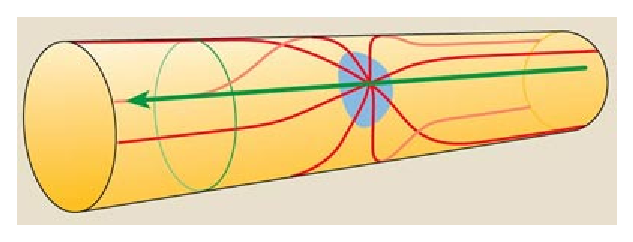
\includegraphics[width=0.6\textwidth]{theory/figures/oneextras1}}
	\caption{Drawing of compactified extra dimensions. 
          The three-dimensional brane lies along the green
          line, while infinite extra dimensions (green circles)
          make up the bulk (picture from the web). \label{fig:compact}}
\end{center}\end{figure}


Many ED models developed in the following years
because of the interesting features of the
basic idea that the Standard Model particles are confined
to our three-dimensional brane.
In general, in most of ED theories Kaluza-Klein (KK) states
appear. These are infinite modes, also called ``towers'', 
existing for every particle
that can propagate to the extra dimensions as resonances.
In other terms, the same particle exists with larger and
larger mass the further goes towards extra dimensions, and
these states can be observed on the three-dimensional brane
(Figure~\ref{fig:tower}).


\begin{figure}[htb]\begin{center}
	\subfigure[]{\label{fig:ed}
  	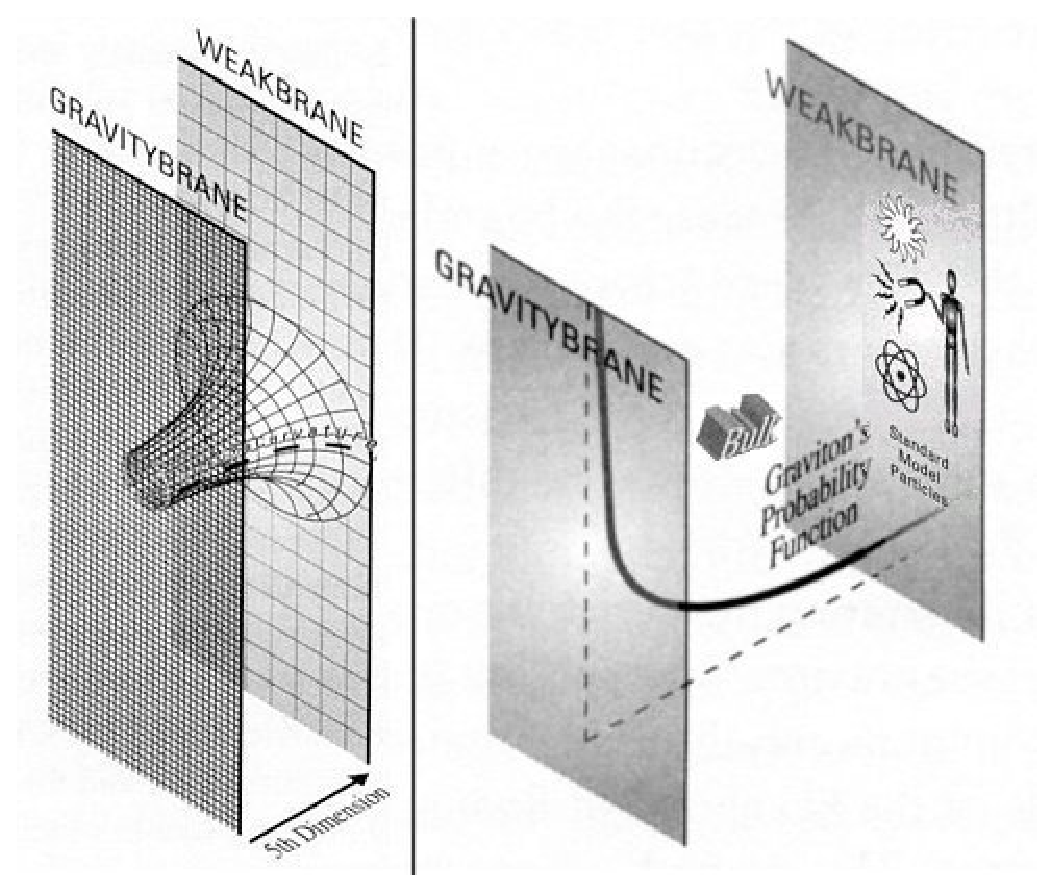
\includegraphics[width=0.4\textwidth]{theory/figures/I15-71-warpedi}}
	\subfigure[]{\label{fig:tower}
  	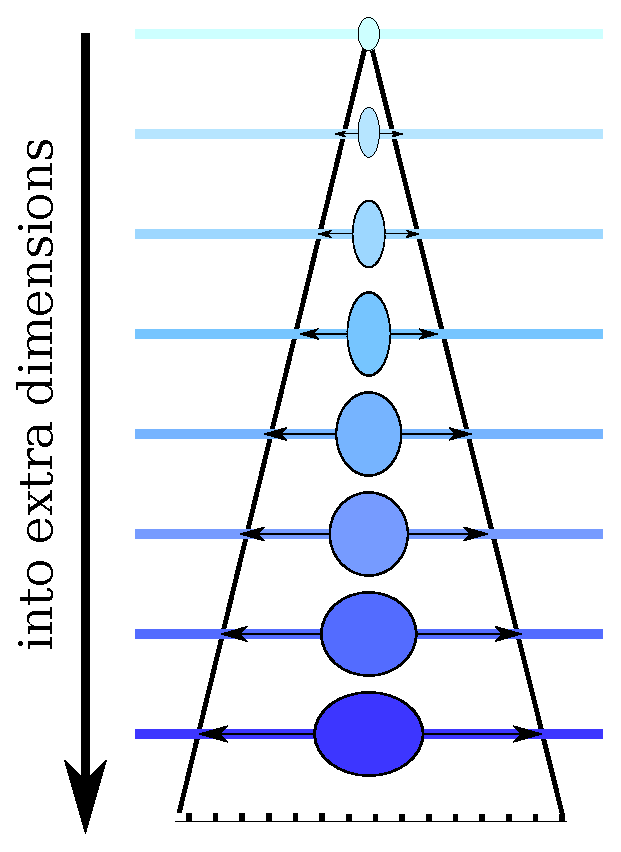
\includegraphics[width=0.3\textwidth]{theory/figures/extradimension}}
	\caption{(a): Pictorial representation of
          the 5th dimension (from \url{http://universe-review.ca}). 
          (b): Pictorial representation of a KK tower, with 
        particles aquiring more mass oscillating towards the
        5th dimension.}
\end{center}\end{figure}
